
\documentclass[a4,10pt]{ctexart}

\usepackage{ctex}
\usepackage[utf8]{inputenc}
\usepackage{amsfonts,amsmath,amscd,amssymb,amsthm}
\usepackage{latexsym,bm}
\usepackage{cite}
\usepackage{mathtools,mathdots,graphicx,array}
\usepackage{fancyhdr}
\usepackage{lastpage}
\usepackage{color}
\usepackage{enumitem}
\usepackage{mpdoc}
\usepackage{diagbox}
\usepackage{xcolor,tcolorbox,tikz,tkz-tab,mdframed,tikz-cd}
\usepackage{framed}
\usepackage{verbatim}
\usepackage{extarrows}
\usepackage{fontspec}
\newcommand*{\dif}{\mathop{}\!\mathrm{d}}
\newcommand*{\arsinh}{\mathop{}\!\mathrm{arsinh}}
\newcommand*{\artanh}{\mathop{}\!\mathrm{artanh}}
\newcommand*{\arcosh}{\mathop{}\!\mathrm{arcosh}}
\newcommand*{\Li}{\mathop{}\!\textrm{Li}}



\begin{document}
\pagenumbering{roman}
\title{随机过程课程作业}
\author{56-丁力-202328015926048}
\date{\today}
\maketitle
\tableofcontents
\newpage
\pagenumbering{arabic}
\newpage

\section{随机过程及其分类}

\begin{ti}{1}{}

    设随机变量 $X$ 服从参数为 1 的指数分布, 随机变量 $Y \sim N(0,1)$, 
    且 $X$ 与 $Y$ 独立, 试求随机变量 $Z=\sqrt{2 X}|Y|$ 的分布密度函数。
\end{ti}
    \begin{qj}
    % 在此处填写答案
    

\end{qj}

    从上我们可以知道, $X$ 服从参数为$\lambda=1$的指数分布, 
    $Y$服从标准正态分布。
    
    那么,我们可以得到两者对应的概率密度函数:

    \begin{align}
        f_{X}(x) &= 
        \begin{cases}
            e^{-x} , x>0 \\
            0, \mbox{其他}
        \end{cases}
                \\
        f_{Y}(y) &= \frac{1}{\sqrt{2\pi}} e^{-\frac{1}{2y^2}}, y \in R
    \end{align}

    
    由于$X$和$Y$相互独立, 所以有:

\begin{equation}
    f_{XY}(x,y) = f_X(x) \times f_Y(y) =\frac{1}{\sqrt{2\pi}}  e^{-x} e^{-\frac{1}{2y^2}}
\end{equation}

                                                                                                                                                                                                                                                                                                                                                                                                                                                                                                                                                                                                                                                                                                                                                                                                                                                                                                                                                                                                             

由于我们知道$\delta$函数具有选择特性, 也就是说:
\begin{equation}
    \int_{-\infty}^\infty \delta(x-a) f(x) \, dx = f(a)
\end{equation}

那么,我们可以得到:
\begin{align}
    f_Z(z) &= \int_0^\infty f(x) dx \int_{-\infty}^\infty f(y) \delta(z-\sqrt{2x}|y|) \, dy \\
    &= \frac{1}{\sqrt{2\pi}} \int_0^\infty e^{-x} dx \int_{-\infty}^\infty e^{-\frac{1}{2y^2}} \delta(z-\sqrt{2x}|y|) \, dy \\
\end{align}
    

由于$\delta$函数具有选择特性, 也就是说:
\begin{equation}
    \int_{-\infty}^{\infty} f(y) \delta(g(y)) \, dy = \sum_{i} \frac{f(y_i)}{|g'(y_i)|}
\end{equation}

那么我可以把(6)式子继续计算:

\begin{align}
    f_Z(z) &= \frac{1}{\sqrt{2\pi}} \int_0^\infty e^{-x} 
    dx \frac{e^{-\frac{y^2}{2}}|_{\frac{z}{\sqrt{2x}}}+e^ {-\frac{y^2}{2}}|_{-\frac{z}{\sqrt{2x}}}} {\sqrt{2x}}\\
    &=\frac{1}{\sqrt{\pi}} \int_0^\infty \frac{e^{-(x^2+\frac{z^2}{4x})}}{\sqrt{x}} dx 
    \end{align}


令$u=\sqrt{x}$, 那么有, 原式为:

\begin{align}
    f_Z(z) &= \frac{2}{\sqrt{\pi}} \int_0^\infty e^{-u^2-\frac{z^2}{4u^2}} \, du \\
    &= \frac{2}{\sqrt{\pi}} \frac{1}{2} e^{-z}\sqrt{\pi} \\
    & = e^{-z},\qquad z>0
    \end{align}

易知,$z<0$, 时, $f_Z(z)=0$。

那么,我们可以得到其概率密度函数为:

\begin{equation}
    f_Z(z) = \begin{cases}
        e^{-z}, z>0 \\
        0, \mbox{其他}
    \end{cases}
\end{equation}



    
    \begin{ti}{2}{}

    设随机变量 $X_1, X_2$ 独立同分布, 服从参数为 $\lambda>0$ 的指数分布, 试证明随机变量
    
    
    \begin{equation}
    \frac{X_1}{X_1+X_2} \sim U[0,1] 
   \end{equation}
    
\end{ti}
    \begin{proof}

    \end{proof}
    % 在此处填写答案
    从上我们可以知道:
    
    \begin{align}
        f_{X_1}(x_1) &=   \begin{cases}
            \lambda e^{-\lambda x_1}, x_1>0 \\
            0, \mbox{其他}\\
        \end{cases} \\
        f_{X_2}(x_2) &=  \begin{cases}
            \lambda e^{-\lambda x_2}, x_2>0 \\
            0, \mbox{其他}\\
        \end{cases}
    \end{align}
    
    
并且,令
\begin{equation}
    Y = \frac{X_1}{X_1+X_2}
\end{equation}

那么有: 
\begin{equation}
    0 < Y < 1
\end{equation}


所以要证明$Y$服从$U[0,1]$的分布,
只需要证明$Y$的分布函数为:
\begin{equation}
    F_Y(y) = \begin{cases}
        0, y\leq 0 \\
        y, 0 < y > 1 \\
        1, y\geq 1
    \end{cases}
\end{equation}

也就是证明其概率密度函数为:
\begin{equation}
    f_Y(y) = \begin{cases}
        1, 0 < y < 1 \\
        0, \mbox{其他}
    \end{cases}
\end{equation}


根据概率分布函数的定义:

\begin{align}
    F_Y(y) &= P(Y \leq y) \\
    &= P(\frac{X_1}{X_1+X_2} \leq y) \\
    &= P(X_1 \leq y(X_1+X_2)) \\
    &= P(X_1 - y(X_1+X_2) \leq 0) \\
\end{align}


令$Z=X_1+X_2$, 那么有:
\begin{align}
    X_1 &= ZY \\
    X_2 &= Z(1-Y)
\end{align}



那么可以得到其对应的Jacobian行列式为:
\begin{equation}
    J = \begin{vmatrix}
        \frac{\partial x_1}{\partial z} & \frac{\partial x_1}{\partial y} \\
        \frac{\partial x_2}{\partial z} & \frac{\partial x_2}{\partial y}
    \end{vmatrix} = \begin{vmatrix}
        y & z \\
        1-y & -z
    \end{vmatrix} = -z
\end{equation}

那么我们可以通过联合概率密度分布通过积分的方式得到其概率密度函数,
首先,我们有:


\begin{align}
   f_{Z,Y}(z,y) &= 
   f_{X1, X2}(x_1, x_2)\times |J| \\
   &= f_{X1, X2}(zy, z(1-y)) \times |J| \\ 
    &= \lambda^2 z e^{-\lambda z}  \\
\end{align}


那么我们可以计算出其边缘概率密度函数为:
\begin{align}
    f_Y(y) &= \int_{0}^\infty f_{Z,Y}(z,y) \, dz \\
    &= \int_{0}^\infty \lambda^2 z e^{-\lambda z} \, dz \\
    \intertext{使用分部积分法,我们可以得到:} 
    &= \lambda^2 \left( -\frac{z e^{-\lambda z}}{\lambda} \bigg|_0^\infty + \int_{0}^\infty \frac{e^{-\lambda z}}{\lambda} \, dz \right) \\
    &= \lambda^2 \int_{0}^\infty \frac{e^{-\lambda z}}{\lambda} \, dz \\
    &= \lambda^2 \left( -\frac{e^{-\lambda z}}{\lambda^2} \bigg|_0^\infty \right) \\
    &= 1
\end{align}


显然,当$y \leq 0$ 或 
$y \geq 1$时, $f_Y(y) = 0$,
至此,我们完成了对于$f_Y(y)= \begin{cases}
    1, 0 < y < 1 \\
    0, \mbox{其他}
    \end{cases}$的证明。
    

    这正是均匀分布 \(U[0,1]\) 的概率密度函数。因此,我们可以得出结论,随机变量

\[
Y = \frac{X_1}{X_1+X_2}
\]

服从 \(U[0,1]\) 分布。至此,我们完成了证明。\\

\(\blacksquare\) Q.E.D 

    
    \begin{ti}{3}{}

    设随机向量 $(X, Y)$ 的两个分量相互独立, 且均服从标准正态分布 $N(0,1)$。
    
    (a) 分别写出随机变量 $X+Y$ 和 $X-Y$ 的分布密度。

\end{ti}

\begin{qj}
由题,可以知道:
\begin{align}
    X &\sim N(0,1) \\
    Y &\sim N(0,1)
\end{align}

由于$X$和$Y$相互独立, 所以有:

\begin{align}
    X+Y &\sim N(0+0, 1+1) \\
    &= N(0,2)\\
    X-Y &\sim N(0-0, 1+1) \\
    &= N(0,2)
\end{align}

所以,我们可以得到其对应的概率密度函数为:
\begin{align}
    f_{X+Y}(x) &= \frac{1}{\sqrt{4\pi}} e^{-\frac{x^2}{4}}, x \in R\\
    f_{X-Y}(x) &= \frac{1}{\sqrt{4\pi}} e^{-\frac{x^2}{4}},x \in R\
\end{align}


\end{qj}


    (b) 试问: $X+Y$ 与 $X-Y$ 是否独立?说明理由。
    
\begin{qj}
    要证明两者独立,也就是证明:
\begin{equation}
    f_{X+Y, X-Y}(x,y) = f_{X+Y}(x) \times f_{X-Y}(y)
\end{equation}


也就是证明上述的联合概率密度函数可以被分解为两个概率密度函数的乘积。

首先我们考虑$X$和$Y$的联合概率密度函数为:

\begin{equation}
    f_{X,Y}(x,y) = \frac{1}{2\pi} e^{-\frac{x^2+y^2}{2}}    
\end{equation}

考虑换元,令:\
\begin{equation}
    \begin{cases}
        u = x+y \\
        v = x-y
    \end{cases}
\end{equation}

那么可以得到:
\begin{equation}
    \begin{cases}
        x = \frac{u+v}{2} \\
        y = \frac{u-v}{2}
    \end{cases}
\end{equation}

其对应的Jacobian行列式为:
\begin{equation}
    J = \begin{vmatrix}
        \frac{\partial x}{\partial u} & \frac{\partial x}{\partial v} \\
        \frac{\partial y}{\partial u} & \frac{\partial y}{\partial v}
    \end{vmatrix} = \begin{vmatrix}
        \frac{1}{2} & \frac{1}{2} \\
        \frac{1}{2} & -\frac{1}{2}
    \end{vmatrix} = -\frac{1}{2}
\end{equation}

那么我们接着计算$X+Y$和$X-Y$的联合概率密度函数:

\begin{align}
    f_{U, V}(u,v) &= f_{X,Y}(x,y) \times |J| \\
    &= f_{X,Y}(\frac{u+v}{2}, \frac{u-v}{2}) \times |J| \\
    &= \frac{1}{2\pi} e^{-\frac{u^2+v^2}{4}} \times \frac{1}{2} \\
    &= \frac{1}{4\pi} e^{-\frac{u^2+v^2}{4}}
\end{align}

从上一题中,
我们可以知道 \(U\) 和 \(V\) 的边缘分布是:

\[
f_U(u) = \frac{1}{\sqrt{4\pi}} e^{-\frac{u^2}{4}}
\]
\[
f_V(v) = \frac{1}{\sqrt{4\pi}} e^{-\frac{v^2}{4}}
\]

现在我们可以尝试将 \(f_{U,V}(u, v)\) 分解为 \(f_U(u) \cdot f_V(v)\):

\[
f_U(u) \cdot f_V(v) = \left( \frac{1}{\sqrt{4\pi}} e^{-\frac{u^2}{4}} \right) \cdot \left( \frac{1}{\sqrt{4\pi}} e^{-\frac{v^2}{4}} \right) = \frac{1}{4\pi} e^{-\frac{u^2+v^2}{4}}
\]

我们可以看到 \(f_{U,V}(u, v)\) 确实可以分解为 \(f_U(u) \cdot f_V(v)\),这意味着 \(U\) 和 \(V\) 是独立的。

所以,我们可以得出结论:\(X+Y\) 和 \(X-Y\) 是独立的随机变量。


\end{qj}


    
    \begin{ti}{4}{}

    设二维随机变量 $(X, Y)$ 的联合密度函数为:
    \begin{equation}
    f(x, y)=\left\{\begin{array}{lc}
    24(1-x) y, & 0<y<x<1 \\
    0, & \text { 其它 }
    \end{array}\right.
   \end{equation}
\end{ti}
    (a) 试求边缘密度函数 $f_X(x)$ 和 $f_Y(y)$, 以及条件密度函数 $f_{X \mid Y}(x \mid y)$ 和 $f_{Y \mid X}(y \mid x)$.


%     {

%     \centering
%     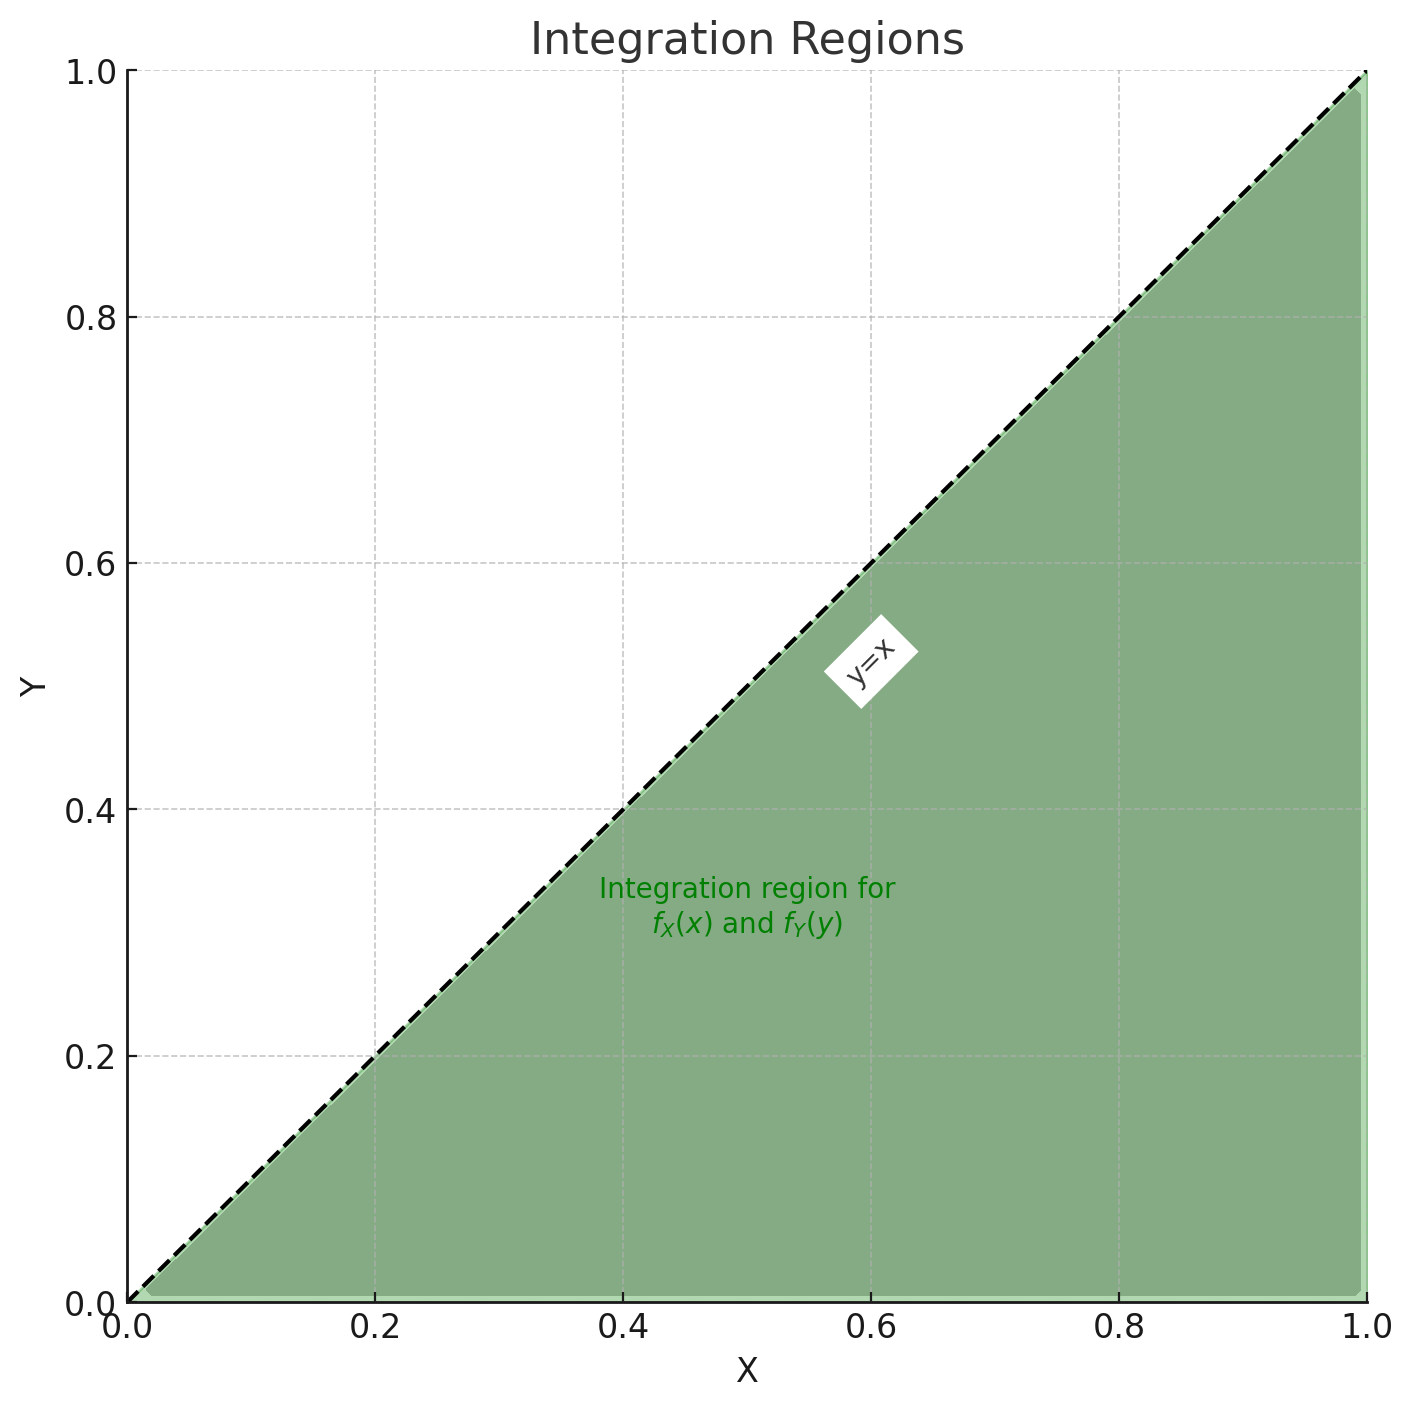
\includegraphics[scale=0.5]{images/1.png}
%     \par

% }

    \begin{qj}
   
    


    由边缘密度函数的定义,可以得到$f_X(x)$:

    \begin{align}
        f_X(x) &= \int_{-\infty}^\infty f_{X,Y}(x,y) \, dy \\
        &= \int_{0}^x 24(1-x)y \, dy \\
        &= 12x^2 - 12x^3 (0<x<1)
    \end{align}



    同理,可以得到$f_Y(y)$:

    \begin{align}
        f_Y(y) &= \int_{-\infty}^\infty f_{X,Y}(x,y) \, dx \\
        &= \int_{y}^1 24(1-x)y \, dx \\
        &= 12y - 24y^2+12y^3 (0<y<1)
    \end{align}

    对于条件密度函数:
    \begin{align}
        f_{X \mid Y}(x \mid y) &= \frac{f_{X,Y}(x,y)}{f_Y(y)} \\
        &= \frac{24(1-x)y}{12y - 24y^2+12y^3} \\
        &= \frac{2(1-x)}{1-2y+2y^2} (0<y<x<1)
    \end{align}


    \begin{align}
        f_{Y \mid X}(y \mid x) &= \frac{f_{X,Y}(x,y)}{f_X(x)} \\
        &= \frac{24(1-x)y}{12x^2 - 12x^3} \\
        &= \frac{2y}{x^2 }, (0<y<x<1)
    \end{align}

    
\end{qj}
   %  \end{qj}
    
    (b) 当 $0<y<1$ 时, 确定 $E\{X \mid Y=y\}$, 以及 $E\{X \mid Y\}$ 的分布密度函数。
    
   \begin{qj}

在求解期望之前, 需要先求得条件概率密度函数$f_{X \mid Y}(x \mid y)$。

这个,我们之前已经求结果,这里直接给出:
\begin{align}
    f_{X \mid Y}(x \mid y) &= \frac{2(1-x)}{1-2y+2y^2} (0<y<x<1)
\end{align}


那么, 对应的期望可以表达为:
\begin{align}
    E\{X \mid Y=y\} &= \int_{-\infty}^\infty x f_{X \mid Y}(x \mid y) \, dx \\
    &= \int_{y}^1 x \frac{2(1-x)}{1-2y+2y^2} \, dx \\
    &=  \frac{2y^3-3y^2+1}{3(1-2y+2y^2)} (0<y<1)
\end{align}


现在,我们来计算$E\{X \mid Y\}$的分布密度函数。
为了计算$E\{X \mid Y\}$的分布密度函数,我们需要先求得$E\{X \mid Y\}$的分布函数。
直接对$E\{X \mid Y\}$的分布函数求导即可得到其分布密度函数。


\begin{align}
    \frac{d}{dy} E\{X \mid Y\} &= \frac{ \frac{2y^3-3y^2+1}{3(1-2y+2y^2)} }{dy} \\
    &= \frac{d}{dy} E\{X \mid Y\} = \frac{2(2y^4 - 4y^3 + 6y^2 - 5y + 1)}{3(4y^4 - 8y^3 + 8y^2 - 4y + 1)}
    (0 < y < 1 )
\end{align}


   \end{qj}
    

% \section{引言}

% 最近闲来无事, 整理了一个写文章看上去比较好用的模板. 

% 你可以对照源代码, 来看一下如何使用这些内容.

% 需要一定的基础. 

% \section{常用环境}
% \begin{yd}{这是一个约定}{}
              
% 约定的内容.
% \end{yd}

% 上述就是一些文本了. 使用的代码是
% \begin{lstlisting}{language=latex}
% \begin{yd}{这是一个约定}{}
              
% 约定的内容.
% \end{yd}
% \end{lstlisting}

% \begin{zs}
        
% 这是一个注释
    
% \end{zs}
    
% \begin{xt}
        
% 这是一个习题.
    
% \end{xt}
    
% \begin{lt}
        
% 这是一个问题.
    
% \end{lt}

% \begin{yl}
        
% 这是一个引理.
    
% \end{yl}

% \begin{dl}{A}{}
        
% 这是一个定理.
    
% \end{dl}
    
% \begin{tl}{A}{}
        
% 这是一个推论.
    
% \end{tl}

% \begin{dy}{A}{}
        
% 这是一个定义.
    
% \end{dy}

% \begin{jl}{A}{}
        
% 这是一个结论.
    
% \end{jl}

% \begin{mt}{A}{}
        
% 这是一个命题.
    
% \end{mt}

% \begin{ti}{A}{}
        
% 这是一个题目.
    
% \end{ti}

% \begin{cx}{A}{}
        
% 这是一个猜想.
    
% \end{cx}

% \begin{zy}
        
% 这是注意.
    
% \end{zy}

% \begin{ts}
        
% 这是一点提示.
    
% \end{ts}

% \begin{lt}
        
% 这是一个例题.
    
% \end{lt}

% \begin{proof}
% 你还可以加一点证明. 
% \end{proof}

% 我们注意到, 所有的数学公式将自动转换成行间公式的大小, 比如${1\over 2^k}$, $\sum_{i=0}^{998244353}i$. 

% \section{起源与未来的修改计划}

% 起源与hkmod的模板, 添加了一些常用的标志词. 可以在mpdoc.sty里面进行更改, 相信根据注释你也会. 

% 使用愉快! 
    
    
    
    
   

\end{document}
